% ===== PDF p.079 (原书 p.71) =====
% 本章原书节号用阿拉伯数字（1, 2, 3, 3.1, 3.2, 3.3, 3.4, 4），与全书多数章用罗马数字不同；
% 按体例在 \chapter 之前切换编号，章末 reflist 之后还原，以免影响后续各章。
\renewcommand{\thesection}{\arabic{section}}

\chapter{镜像对称与共形场论}
\chapterauthor{細野忍}{[東京大学大学院数理科学研究科]}

\section{引言}

前面几章已经说明：人们从弦理论的研究中发现了 Calabi--Yau 流形上的镜像对称，物理学家与数学家共同开展研究，在代数几何与辛几何的交界处取得了许多成果。

这里，我想从物理学家描述弦理论所用的手段——共形场论——这一视角出发，稍微深入镜像对称的某一个侧面，试着作一点解说。

镜像对称的关键在于共形场论，具体说是称为 $N=2$ 共形场论的东西。第 1 章已经对它作了清晰明快的讲解，所以这里从路径积分给出的等价表述开始。

\section{什么是弦理论}

做数学时，谁都会觉得：不先把定义弄清楚，讨论就无法推进。于是一开始大概就会有人问：“弦理论的定义是什么？”不过，这里我们暂且把下面这样的东西当作一个定义，开始讨论。

取紧致的 $C^\infty$ 流形 $X$，取亏格（genus）为 $g$ 的黎曼面 $\Sigma_g$。在 $X$ 上给定度量 $G_{AB}$，在 $\Sigma_g$ 上给定度量 $h_{ab}$。这时，对 $C^\infty$ 映射 $\phi\colon\Sigma_g\to X$ 与度量 $h_{ab}$ 赋以适当的权重，把所有情形“求和”起来，即
\begin{equation}
  F_g^X(G) := \int \mathcal{D}h_{ab}\int \mathcal{D}\phi\; e^{-S(h,\phi;G)}
  \tag{1}
\end{equation}
我们称之为 $X$ 上的弦理论。这里，$\int\mathcal{D}h_{ab}\int\mathcal{D}\phi$ 表示对全体度量 $h_{ab}$ 与全体 $C^\infty$ 映射所成的无穷维空间作积分；物理学中把它叫作 Feynman 路径积分。

% ===== PDF p.080 (原书 p.72) =====
对数学家来说，路径积分这种东西一上来就显得有些可疑。但 20 世纪的理论物理学、尤其是量子场论，缺了它便无从谈起。所幸在 (1) 的情形，我们能够导出更像样的积分形式。于是，把表示权重的函数 $S(G)=S(h,\phi;G)$ 定为
\begin{equation}
  S(G)=\frac{1}{4\pi}\int_{\Sigma_g} d^2x\,\sqrt{h}\,G_{AB}h^{ab}
  \frac{\partial\phi^A}{\partial\theta^a}\frac{\partial\phi^B}{\partial\theta^b}
  \tag{2}
\end{equation}
这样的形状。这里，在 $\Sigma_g$ 上取局部坐标 $(\theta^a)=(\theta^1,\theta^2)$，在 $X$ 上同样取局部坐标，并用这些坐标表示 $C^\infty$ 映射 $\phi\colon\Sigma_g\to X$。另外，$(h^{ab})=(h_{ab})^{-1}$，$h=\det h_{ab}$；重复的指标在没有特别说明时表示求和，这就是 Einstein 求和约定。

权重函数 $S(h,\phi;G)$ 自然在 $\Sigma_g$ 的坐标变换 $\theta^a\to\theta^a+\xi^a(\theta)$ 下不变。不仅如此，它在度量 $h_{ab}$ 的共形变换
\[
  h_{ab}(\theta)\longrightarrow e^{\rho(\theta)}h_{ab}(\theta)
\]
下也不变，这就定义了标题所说的共形场论。共形场论的特点是：关于全体度量 $h_{ab}$ 的求和缩小为
\[
  \mathcal{M}_g=\{\ \Sigma_g \text{ 上的度量 } h_{ab}(\theta)\ \}/\sim
\]
这里，$\sim$ 的意思是：由坐标替换或共形变换联系起来的度量看作同一个，只数一次。$\mathcal{M}_g$ 作为黎曼面复结构的形变空间（黎曼面的模空间）已有细致研究，特别地，人们知道它是紧致复流形（$\dim_{\C}\mathcal{M}_g=3g-3$，$g>1$）。这样，两个路径积分中的一个便换成有限维积分，得到
\begin{equation}
  F_g^X(G)=\int_{\mathcal{M}_g} d^{6g-6}m\int\mathcal{D}\phi\; e^{-S(h,\phi;G)}
  \tag{3}
\end{equation}
路径积分仍然留在式子里，还不能算数学定义，但对物理学家来说已是足够的定义。因为以它为基础的计算处方确实存在。但下面两点很重要，这里只提结论、细节从略：

% ===== PDF p.081 (原书 p.73) =====
1) 路径积分 $\int\mathcal{D}h_{ab}$ 实际缩小为模空间 $\mathcal{M}_g$ 上的积分，是在流形 $X$ 的 Ricci 曲率 $R(G)_{AB}$ 等于 0 的情形。准确地说，需要 10 维的是整体流形；这里把它理解为 $\R^{d-1,1}\times X$ 这样的 10 维流形，由 $d$ 维时空与 $X$ 的直积给出。

2) 式 (1)、(3) 中省略了，但（超）弦理论考虑的是同时具有玻色子与费米子对称性的设定。其结果，要求 $X$ 是 Kähler 流形。

在 1)、2) 的要求之下，我们到达这样的流形：它是紧致 Kähler 流形，并且具有 Ricci 曲率 $R(G)_{i\bar j}=\partial_i\partial_{\bar j}\det(G_{m\bar n})$ 等于零的度量 $G_{i\bar j}$（Calabi--Yau 度量）——这就是 Calabi--Yau 流形。
% [Tutor Note: 原书此处写作 $R(G)_{i\bar j}=\partial_i\partial_{\bar j}\det(G_{m\bar n})$，照录原文；通常 Ricci 形式写作 $R_{i\bar j}=-\partial_i\partial_{\bar j}\log\det(G_{m\bar n})$。]

\section{镜像对称}

弦理论中，固定复 $n$ 维 Calabi--Yau 流形 $X$，考虑其 Calabi--Yau 度量 $G_{AB}$ 的函数 $F_g^X(G)$。这里，我们来考虑 Calabi--Yau 度量 $G_{AB}$ 的形变，考察函数 $F_g^X(G)$ 的性质。

\subsection{形变的参数与镜像对称}

$X$ 是复流形时，存在满足 $J^2=-1$ 的张量 $J^A_{\ B}$（复结构）。把度量 $G_{AB}$ 取成 Hermite 型，则 $G_{AB}=G_{CD}J^C_{\ A}J^D_{\ B}$ 成立，$K_{AB}=G_{AC}J^C_{\ B}$ 成为反对称的 $K_{AB}=-K_{BA}$，从而确定 2 次微分形式 $K$。使 $K$ 成为闭形式的度量叫作 Kähler 度量；具有这种度量的复流形叫作 Kähler 流形。$K$ 确定 2 次上同调类 $[K]\in H^2(X,\R)$；像这样由 Kähler 度量的类 $[K]$ 表示的上同调类，叫作 Kähler 类。带有 Ricci 张量 $R(G)_{AB}$ 等于 0 的 Kähler 度量的 Kähler 流形，就是前一节出现的 Calabi--Yau 流形。

切丛的第一 Chern 类 $c_1(X)$ 用 Ricci 张量表示，所以 Calabi--Yau 流形满足 $c_1(X)=0$。反过来，著名的 Yau 定理说：“在满足 $c_1(X)=0$ 的紧致 Kähler 流形 $X$ 上，给定 Kähler 类 $\mu$，则存在唯一的 Kähler 度量满足 $R(G)_{AB}=0$。”
% ===== PDF p.082 (原书 p.74) =====
根据这个定理，人们常把满足 $c_1(X)=0$ 的紧致 Kähler 流形定义为 Calabi--Yau 流形。另外，条件 $c_1(X)=0$ 也可以换个说法：典范丛 $K_X$ 平凡。

那么，Calabi--Yau 度量写作 $G_{AB}=-K_{AC}J^C_{\ B}$，我们来考虑它的微小形变。首先，复结构 $J$ 的形变可用 Kodaira--Spencer 的复流形形变理论。按该理论，无穷小形变由以全纯切丛 $T'X$ 为系数的 1 次上同调 $H^1(X,T'X)$ 给出。在 Calabi--Yau 流形的情形，幸运的是，这些无穷小形变全都能延拓到微小的有限邻域。结果，作为微小形变的参数，可以取 $s=\dim_{\C}H^1(X,T'X)$ 个（复）坐标
\[
  J^A_{\ B}(m)=J^A_{\ B}(m_1,\dots,m_s)
\]
另一方面，Kähler 形式 $K_{AB}$ 由 Yau 定理保证：只要作为 $H^2(X,\R)$ 的元素给定 Kähler 类 $[K]$，它就唯一确定。于是，取 $H^2(X,\R)$ 的线性实坐标 $\lambda_1,\dots,\lambda_r$，就可以把形变参数写成
\[
  K_{AB}(\lambda)=K_{AB}(\lambda_1,\dots,\lambda_r)
\]
对 Calabi--Yau 流形 $X$ 定出的弦理论 $F_g^X(G)$，就是这些有限个参数的函数。

Kähler 形式的形变参数是实变量 $\lambda$，但若把称为 B-field 的场也包括进来，则已知它自然地收纳在复变量 $t_i=b_i+\sqrt{-1}\lambda_i$ 的虚部中。变量 $t_i$ 叫作复化 Kähler 参数，是表示 $H^2(X,\R)+\sqrt{-1}H^2(X,\R)$ 的元素 $B+\sqrt{-1}K$ 的线性参数。与这一扩充相应，弦理论 $F_g^X(G)$ 被稍作修改为 $F_g^X(G,B)$。

对 $X$ 直接计算并确定弦理论 $F_g^X(G,B)$ 几乎不可能。但是，1986 年物理学家 Gepner 发现了一种方法：用 $N=2$ 共形场论，严格求出与某些 $X$ 及其特殊度量 $(G_0,B_0)$ 相对应的、被认为是 $F_g^X(G_0,B_0)$ 的量。当时，它作为弦理论的严格解引起了许多物理学家的兴趣；由这类研究，人们在 1990 年前后明确认识到了下面的现象——镜像对称。

\noindent\textbf{镜像对称猜想}\quad 取 Calabi--Yau 流形 $X$，定出弦理论 $F_g^X(G_X,B_X)$。此时，
\begin{equation}
  F_g^X(G_X,B_X)=F_g^Y(G_Y,B_Y)
  \tag{4}
\end{equation}
% ===== PDF p.083 (原书 p.75) =====
成立，并且存在这样的 Calabi--Yau 流形 $Y$ 与 $(G_Y,B_Y)$，以及两者形变的局部参数之间的可逆全纯函数
\begin{equation}
\begin{array}{ll}
  t_i^X=\Phi_i(m_1^Y,\dots,m_r^Y) & (i=1,\dots,r)\\[2pt]
  m_k^X=\Psi_k(t_1^Y,\dots,t_s^Y) & (k=1,\dots,s)
\end{array}
\tag{5}
\end{equation}

这里，关系式 (5) 叫作镜像映射。
% [Tutor Note: 「ミラー写像」译作「镜像映射」，与「ミラー変換」（镜像变换）分工：后者指两边的变换关系，前者指具体的那组映射。]

Calabi--Yau 流形上 $K_X$ 平凡，结合 Serre 对偶可得 $\dim_{\C}H^1(X,T'X)=h^{n-1,1}(X)$，所以（5）式包含 Hodge 数的关系
\[
  h^{1,1}(X)=h^{n-1,1}(Y),\qquad h^{n-1,1}(X)=h^{1,1}(Y)
\]
第 4 章说过，Calabi--Yau 流形究竟有多少种，这个高维代数流形的分类问题至今仍未解决；从这个观点看，也可以说镜像对称是有趣的猜想。

\subsection{实 2 维环面的例子}

按第 1 节给出的“像是定义的东西”实际计算弦理论，几乎不可能。但是，$X$ 是实 $2n$ 维环面时，可以依照定义“忠实地”计算出来。其结果由具有 $(2n,2n)$ 型符号的偶自对偶格——Narain 格完全描述。下面介绍最简单的 $n=1$ 的情形作为例子。
% [Tutor Note: 原书两处均写作“第 1 节”，但下文所指的“像是定义的东西”实际出现在第 2 节《什么是弦理论》中；这是底本的指代疏漏，译文照录不改。]

如图 1 所示，在实坐标为 $(\phi^1,\phi^2)$ 的环面上引入复结构 $T=T_1+iT_2$，把对应的复坐标记为 $w=\phi^1+T\phi^2$。另外，给出 Kähler 形式 $\kappa=\frac{i}{2}\frac{U_2}{T_2}dw\wedge d\bar w=U_2\,d\phi^1\wedge d\phi^2$，与 B-field 合起来，由 $B+i\kappa=(U_1+iU_2)d\phi^1\wedge d\phi^2$ 把复化 Kähler 参数定为 $U=U_1+iU_2$。

\begin{figure}[htbp]
  \centering
  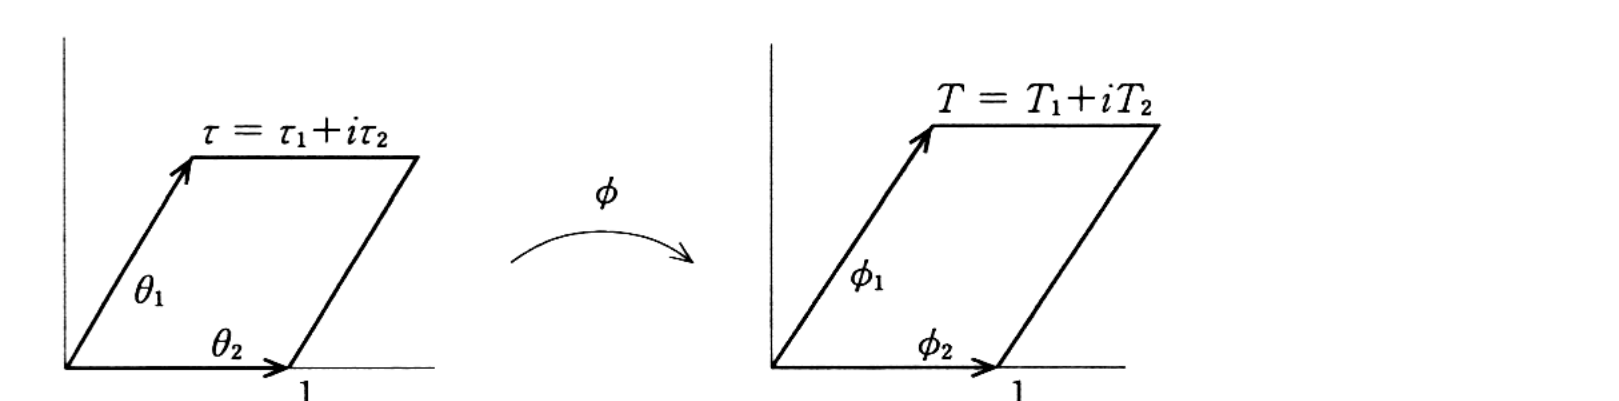
\includegraphics[width=0.75\linewidth]{figures/ch06-fig1.png}
  \figtitle{1}{$C^\infty$ 映射 $\phi\colon\Sigma_1\to X=E_{T,U}$。左为 $\Sigma_1$ 上的复结构 $\tau=\tau_1+i\tau_2$，右为 $X$ 上的复结构 $T=T_1+iT_2$（原书 p.75）}
\end{figure}

% ===== PDF p.084 (原书 p.76) =====
把这两种结构一并放入的环面记为 $X=E_{T,U}$。另一方面，用格把 $X$ 表示成
\[
  X=\R^2/2\pi\Lambda_{\Z}
\]
这里，$\Lambda_{\Z}$ 是由
\begin{equation}
  (\xi_1,\xi_2)=\sqrt{\frac{U_2}{T_2}}
  \begin{pmatrix} 1 & T_1\\ 0 & T_2\end{pmatrix}
  \tag{6}
\end{equation}
定出的向量 $\xi_1,\xi_2$ 生成的格。这时，复结构 $T$ 与 Kähler 形式 $\kappa$ 定出的度量为 $G_{ij}=\xi_i\cdot\xi_j$。

同样，在实坐标为 $\theta^1,\theta^2$ 的 $\Sigma_1$ 上引入复结构 $\tau=\tau_1+i\tau_2$ 与 Kähler 形式 $d\theta^1\wedge d\theta^2$，则 $\Sigma_1$ 的度量为
\[
  (h_{ab})=\frac{1}{\tau_2}
  \begin{pmatrix} 1 & \tau_1\\ \tau_1 & |\tau|^2\end{pmatrix}
\]
由以上数据写出权重函数 (2)，得
\[
  S=\frac{1}{4\pi}\int d^2\theta\,\frac{1}{\tau_2}
  (\tau\partial_1-\partial_2)\phi^i(\bar\tau\partial_1-\partial_2)\phi^j G_{ij}
\]
（$\partial_i:=\partial/\partial\theta^i$）。路径积分要对“全体 $C^\infty$ 映射”进行，但可以像下面这样赋予意义并执行。首先，把 $C^\infty$ 映射 $\phi\colon\Sigma_1\to X$ 用 Fourier 级数表示如下（$0\le\theta^i\le1$）：
\[
  \phi^i(\vec\theta)=2\pi(n_i\theta^1+m_i\theta^2)
  +\sum_{k,l}a_{kl}^{(i)}e^{2\pi\sqrt{-1}(k\theta^1+l\theta^2)}
\]
这里，$\phi(\vec\theta)=\phi^1(\vec\theta)\xi_1+\phi^2(\vec\theta)\xi_2$ 表示 $X=\R^2/2\pi\Lambda_{\Z}$ 上的点，所以系数满足实条件 $\bar a_{kl}^{(i)}=a_{-k,-l}^{(i)}$；另外，整数向量
\[
  \vec n=(n_1,n_2),\qquad \vec m=(m_1,m_2)
\]
表示 $\Sigma_1$ 的 1 维闭链在 $X$ 上缠绕的次数。这样表示时，路径积分 $\int\mathcal{D}\phi$ 按
\[
  \resizebox{0.97\linewidth}{!}{$\displaystyle
  \sum_{\vec n,\vec m}\int\prod_i\prod_{k>0,\,l}
  \frac{da_{kl}^{(i)}\,d\bar a_{kl}^{(i)}}{2\pi\sqrt{-1}}
  \times\prod_{l>0}\frac{da_{0l}^{(i)}\,d\bar a_{0l}^{(i)}}{2\pi\sqrt{-1}}
  \,da_{00}^{(i)}$}
\]
赋予意义。这时，积分容易执行，途中出现的无限乘积也能自然处理。这种路径积分的定义与无限乘积的处理，在共形场论中屡屡出现。
% ===== PDF p.085 (原书 p.77) =====
下面把主要式子展示出来，建议读者当作练习动手计算，体会这套计算处方是如何自然确定的。

用 $\phi^i(\vec\theta)$ 的 Fourier 级数，$S(h,\phi;G)$ 可表为
\[
  S=S_{\vec n,\vec m}+\frac{2\pi}{\tau_2}\sum_{k,l}|\tau k-l|^2
  a_{kl}^{(i)}\bar a_{kl}^{(i)}\xi_i\cdot\xi_j
\]
这里，右边第 1 项来自缠绕，由 $S_{\vec n,\vec m}=\frac{1}{\tau_2}G_{ij}(\tau n_i-m_i)(\bar\tau n_j-m_j)$ 给出。作变量变换
\[
  a_{kl}^{(i)}\xi_i:=\sqrt{U_2}
  \begin{pmatrix} z_{kl}^{(1)}\\ z_{kl}^{(2)}\end{pmatrix}
\]
则权重函数 $S$ 成为
\[
  S_{\vec n,\vec m}+\frac{2\pi}{\tau_2}\sum_{k,l}|\tau k-l|^2U_2
  \bigl(z_{kl}^{(1)}\bar z_{kl}^{(1)}+z_{kl}^{(2)}\bar z_{kl}^{(2)}\bigr)
\]
于是积分归结为 Gauss 积分
\[
  \int\frac{d\bar z\,dz}{2\sqrt{-1}}e^{-A\bar zz}
  =\int dxdy\,e^{-A(x^2+y^2)}=\frac{\pi}{A}
\]
结果，除 $\sum_{\vec n,\vec m}da_{00}^{(1)}da_{00}^{(2)}e^{-S_{\vec n,\vec m}}$ 之外，还得到下面的无限乘积：
\begin{equation}
  \left\{\prod_{k>0,\,l}\frac{\tau_2}{2\pi U_2|\tau k-l|^2}
  \prod_{l>0}\frac{\tau_2}{2\pi U_2l^2}\right\}^2
  \tag{7}
\end{equation}
像重整化理论中常见的那样，场论里会出现各种类型的无穷大，物理学家很熟悉这类无穷大的处理。尤其是上面这个无限乘积的处理，在其中属于最容易的一种，用下面的公式处理：
\[
  \prod_{n=1}^{\infty}\Bigl(1-\frac{z^2}{\pi^2n^2}\Bigr)=\frac{\sin z}{z},
  \qquad
  \prod_{n=1}^{\infty}\frac{\beta}{2\pi n^2}=\frac{1}{\sqrt{2\pi\beta}}
\]
第 1 式是分析学中出现的公式；第 2 式则是用 zeta 函数
\[
  \zeta\Bigl(s,\Bigl\{\frac{\beta}{2\pi n^2}\Bigr\}\Bigr)
  :=\sum_{n>0}\Bigl(\frac{\beta}{2\pi n^2}\Bigr)^{-s}
\]
定义的值 $\prod_{n>0}\frac{\beta}{2\pi n^2}=e^{-\zeta'(0,\{\frac{\beta}{2\pi n^2}\})}$。用这些值把关于 $l$ 的无限乘积按 $l>0$ 与 $l<0$ 合并处理，则由 (7) 式得
\[
  \frac{U_2}{2\pi\tau_2}\Bigl|\prod_{k>0}\frac{e^{\pi ik\tau}}{1-e^{2\pi ik\tau}}\Bigr|^4
  =\frac{U_2}{2\pi\tau_2}\frac{1}{|\eta(\tau)|^4}
\]

% ===== PDF p.086 (原书 p.78) =====
得到。这里，再次作无限和的处理 $\sum_{k>0}k=\zeta(-1)=-\frac{1}{12}$。出现的函数 $\eta(\tau)=q^{\frac{1}{24}}\prod_{n>0}(1-q^n)$（$q=e^{2\pi i\tau}$）叫作 Dedekind 的 $\eta$ 函数，它满足 $\eta(-1/\tau)=\sqrt{\tau/i}\,\eta(\tau)$，而 $\eta^{24}(\tau)$ 是权为 12 的模形式。

归纳以上，作为 $X=E_{T,U}$ 上的弦理论，得到
\begin{equation}
  F_{g=1}^X=\int_{\mathcal{F}}\frac{d\tau\,d\bar\tau}{\tau_2^2}
  \frac{\sqrt{\det G}}{\tau_2|\eta(\tau)|^4}
  \sum_{\vec n,\vec m}e^{-S_{\vec n,\vec m}(G,B)}
  \tag{8}
\end{equation}
这里，关于常值映射的积分 $\frac{1}{2\pi}\int da_{00}^{(1)}da_{00}^{(2)}$ 被省略了。另外，此前一直藏着的 B-field 也若无其事地登场了。B-field 出现在
\[
  S_{\vec n,\vec m}(G,B)=\frac{1}{\tau_2}(G_{ij}+B_{ij})
  (\tau n_i-m_i)(\bar\tau n_j-m_j)
\]
之中。

以上不过是环面这种最容易的情形的计算例，但足以提供动机，让人认真考虑第 1 节给出的“像是定义的东西”。

\subsection{镜像对称与 T 对偶性}

$X=E_{T,U}$ 的情形下 $F_{g=1}^X(G,B)$ 已经确定，所以来找与它镜像对称的 $F_{g=1}^Y(G_Y,B_Y)$ 吧。其实复 1 维 Calabi--Yau 流形只有环面（椭圆曲线），所以此时 $Y$ 只得与 $X$ 一致。不过，镜像对称可由 T 对偶这一几何操作来说明——获得这一洞察，本身就是一个重要的例证。

(8) 式中出现的和 $\sum_{\vec n,\vec m}$ 来自 $\Sigma_1$ 的 1 维闭链在 $X=\R/2\pi\Lambda_{\R}$ 上缠绕数的映射。
% [Tutor Note: 此处原书写作 $\R/2\pi\Lambda_{\R}$，p.76 则写作 $\R^2/2\pi\Lambda_{\Z}$；两处均照录，疑为笔误。]
我们把表示缠绕数的向量 $(\vec n,\vec m)$ 看作 $\Lambda_{\Z}\oplus\Lambda_{\Z}$ 的元素。这里，对两个格中的一个格作“Fourier 变换”，和就换成关于格 $\Lambda_{\Z}^*\oplus\Lambda_{\Z}$ 的和。这可用称为 Poisson 求和公式的等式
\[
  \sum_n e^{-\pi an^2+2\pi ibn}=\frac{1}{\sqrt{a}}\sum_m e^{-\frac{\pi(m-b)^2}{a}}
\]
执行。用这个公式整理 (8) 式，得
\begin{equation}
  \int_{\mathcal{F}}\frac{d\tau\,d\bar\tau}{\tau_2^2}\frac{1}{|\eta(\tau)|^4}
  \sum_{p\in\mathcal{N}_{2,2}}q^{\frac{1}{2}p_L^2}\bar q^{-\frac{1}{2}p_R^2}
  \tag{9}
\end{equation}

% ===== PDF p.087 (原书 p.79) =====
得到。这里出现的 $\mathcal{N}_{2,2}$ 叫作 Narain 格，它是在带 $(2,2)$ 型 Lorentz 内积的向量空间 $\R^{2,2}$ 中、由
\begin{equation}
  (\mathbf{e}_1,\mathbf{e}_2,\mathbf{e}_3,\mathbf{e}_4)=\mathbf{E}
  \begin{pmatrix} {}^t\Xi^{-1} & -B\\ 0 & \Xi\end{pmatrix}
  \tag{10}
\end{equation}
定出的基 $\mathbf{e}_i$ 生成的格。不过，
\[
  \Xi=\sqrt{\frac{U_2}{T_2}}
  \begin{pmatrix} 1 & T_1\\ 0 & T_2\end{pmatrix},
  \qquad
  B=\begin{pmatrix} 0 & U_2\\ -U_2 & 0\end{pmatrix}
\]
而特别地，$\Xi=(\xi_1,\xi_2)$ 与确定格 $\Lambda_{\Z}$ 的基的矩阵 (6) 一致。

此外，用 $\mathbf{E}=\frac{1}{\sqrt{2}}\begin{pmatrix}1&1\\-1&1\end{pmatrix}$ 把基稍微旋转了一下。(9) 中出现的和 $\sum_{p\in\mathcal{N}_{2,2}}$ 里，按向量空间的直和分解 $\R^{2,2}=\R^{2,0}\oplus\R^{0,2}$ 分解 $p$，分别决定射影成分 $p_L,p_R$（$p=(p_L,p_R)$）。

上面矩阵的块中出现的 ${}^t\Xi^{-1}$ 确定对偶格 $\Lambda_{\Z}^*$ 的基，所以可知 $B=0$ 时 Narain 格与 $\Lambda_{\Z}^*\oplus\Lambda_{\Z}$ 一致。直和 $\Lambda_{\Z}^*\oplus\Lambda_{\Z}$ 上，由 $\Lambda_{\Z}^*$ 与 $\Lambda_{\Z}$ 的对偶形式自然带进 $(2,2)$ 型 Lorentz 内积；已知这样的格与 $(1,1)$ 型双曲格 $H$ 的直和 $H^{\oplus 2}$ 同型。有 B-field 时，Narain 格会从直和 $\Lambda_{\Z}^*\oplus\Lambda_{\Z}$ 稍许偏离，但关于 $\R^{2,2}$ 中的 Lorentz 内积，
\[
  \mathbf{e}_1\cdot\mathbf{e}_3=\mathbf{e}_2\cdot\mathbf{e}_4=1
\]
\[
  \mathbf{e}_i\cdot\mathbf{e}_j=0\qquad(\text{其他 } i\le j)
\]
成立，所以 $\mathcal{N}_{2,2}\cong H^{\oplus 2}$。

这个内积的性质表示：矩阵 (10) 属于关于 Lorentz 内积的正交矩阵群 $O(2,2;\R)$。另外，弦论 (9) 显然在分解 $\R^{2,2}=\R^{2,0}\oplus\R^{0,2}$ 下不变，保持它的群作用 $O(2;\R)\times O(2;\R)$ 从左侧作用于矩阵 (10)。进而，以整数为成分的正交矩阵 $O(2,2;\Z)$ 作为 Narain 格的同型从右侧作用于矩阵 (10)。由以上可知，确定基的 (10) 所含的 4 个参数 $T_1,T_2,U_1,U_2$ 可理解为
\[
  \mathcal{M}_{2,2}=O(2;\R)\times O(2;\R)\backslash O(2,2;\R)/O(2,2;\Z)
\]
的坐标。这里出现的正交群及其商，是称为 IV 型对称域的东西的一例，这种情形特别容易，可以证明它等于两个上半平面的直积
\[
  O(2;\R)\times O(2;\R)\backslash O(2,2;\R)\cong\mathbf{H}_+\times\mathbf{H}_+
\]
这 2 个上半
% ===== PDF p.088 (原书 p.80) =====
平面的复坐标不外是 $T=T_1+iT_2$，$U=U_1+iU_2$。关于表示 Narain 格同型的群 $O(2,2;\Z)$，也证明了它由分别作用在各上半平面上的 $PSL(2,\Z)$ 与
\begin{equation}
\begin{aligned}
  (T,U)&\longmapsto(-\bar T,-\bar U),\\
  (T,U)&\longmapsto(U,T)
\end{aligned}
\tag{11}
\end{equation}
生成 [3]。同型群 $O(2,2;\Z)$ 叫作 T 对偶群。这个群是 Narain 格的同型群，所以弦理论 $F_{g=1}^X(G,B)$ 在其作用下不变。

这里，我们来几何地解释 T 对偶群的作用。首先，作用于 $T$ 的 $PSL(2,\Z)$ 是作用于环面复结构的模变换（由 Dehn twist 生成）。另外，(11) 的第 1 式的作用改变 $X=E_{T,U}$ 的 Kähler 形式 $\kappa$ 的符号，所以可理解为把 $X$ 的定向反转的作用。然而，(11) 的第 2 式交换复结构 $T$ 与复化 Kähler 形式参数 $U$，这样的作用在 $X$ 的几何中无法（封闭地）解释。

为了直观理解 T 对偶变换 $(T,U)\leftrightarrow(U,T)$ 在 $X$ 的几何中无法封闭解释的样子，考虑
\[
  T_2=\frac{R_2}{R_1},\qquad U_2=R_1R_2,\qquad T_1=U_1=0
\]
这一特殊情形。此时可知，问题中的变换由 $R_1\mapsto\frac{1}{R_1}$ 表示。另外，$X$ 的度量为
\[
  (G_{ij})=(\xi_i\cdot\xi_j)=
  \begin{pmatrix} R_1^2 & 0\\ 0 & R_2^2\end{pmatrix}
\]
成为半径分别为 $R_1,R_2$ 的圆周 $S^1$ 的直积。把一个圆周写作 $S^1=\R/2\pi R_1\Z$ 时，其对偶圆周由 $(S^1)^\vee=\R/\bigl(2\pi\frac{1}{R_1}\Z\bigr)$ 定出。请观察图 2，体会变换 $R_1\mapsto\frac{1}{R_1}$ 表示镜像对称。
% [Tutor Note: T 对偶是弦论的对称性：半径 $R$ 的圆周与半径 $1/R$ 的圆周给出同一个弦理论（此处取 $\alpha'=1$），故 $R_1\mapsto 1/R_1$ 不改变物理。]

这样，问题中的 T 对偶变换虽然与 $X$ 的几何学毫不相干，却可以理解为一种几何操作。把 $X$ 表示为以环面为纤维的纤维空间，并把纤维中出现的（实）环面全部换成对偶环面。此时，由此再次得到 2 维环面 $Y$，它与 $X$ 的
% ===== PDF p.089 (原书 p.81) =====
镜像对称 Calabi--Yau 流形一致。
\begin{figure}[htbp]
  \centering
  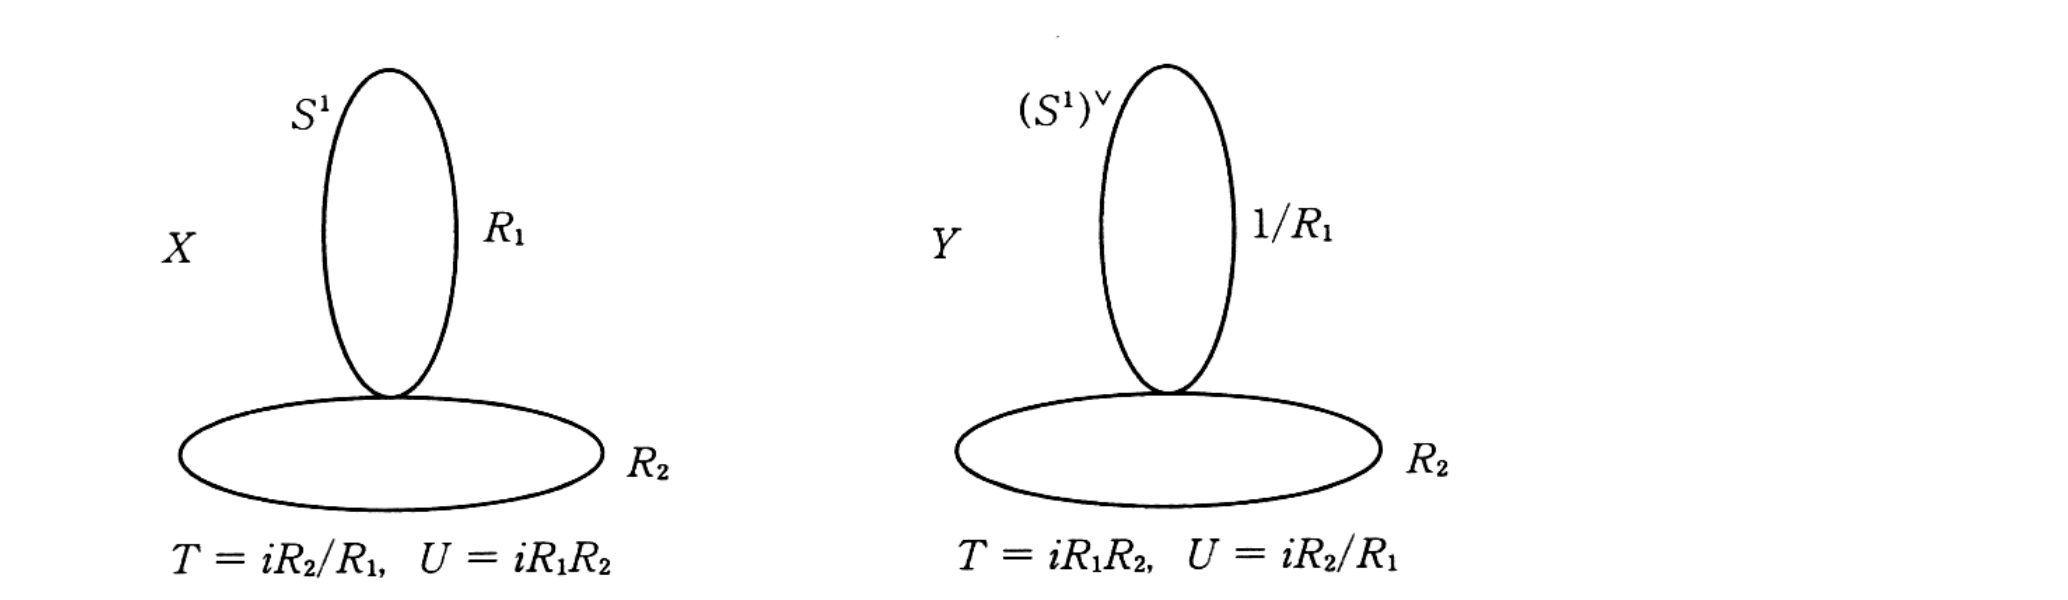
\includegraphics[width=0.85\linewidth]{figures/ch06-fig2.png}
  \figtitle{2}{$T$ 对偶变换 $R_1\mapsto 1/R_1$ 的几何图像。左为 $X$，纵向圆周 $S^1$ 的半径为 $R_1$、横向圆周半径为 $R_2$；右为镜像流形 $Y$，纵向圆周换成对偶圆周 $(S^1)^\vee$，半径为 $1/R_1$，横向仍为 $R_2$（原书 p.81）}
\end{figure}

Strominger--Yau--Zaslow [4] 于 1996 年提出一个想法并引起关注：这种基于纤维空间的图像对高维 Calabi--Yau 流形也成立，由此可以确定镜像对称的 $Y$。如今这个想法已被广泛接受，并以三人的名字称为 SYZ 构造（猜想）。在 SYZ 构造中，要求把 $X$ 表为纤维空间时所用的（实）环面是特殊 Lagrangian 子流形，所以问题变得格外困难。它横跨复几何与辛几何，作为重大的未解决问题，今后的发展值得期待。

\subsection{全纯曲线的计数}

作为镜像对称的重要应用，有 Calabi--Yau 流形的全纯曲线计数问题。量子上同调与 Gromov--Witten 不变量已经解说过，所以这里想把它与弦理论的“像是定义的东西”联系起来。弦理论 $F_g^X(G,B)$ 由关于 $C^\infty$ 映射 $\phi\colon\Sigma_g\to X$ 的路径积分 $\int\mathcal{D}\phi$ 与模空间上的积分 $\int d^{6g-6}m$ 构成。因此，通过适当的操作把关于 $C^\infty$ 映射的和缩小为关于全纯映射 $\phi\colon\Sigma_g\to X$ 的和，就可以作全纯曲线的计数。这听起来像是便宜行事的说法，但把路径积分这样缩小的一般讨论是 Witten [5] 作出的，称为拓扑场论或拓扑极限。粗略地说，它是利用本章省略的费米子与玻色子的对称性，让两者相互抵消、只取出目的部分的操作。

对 $X=E_{T,U}$ 的情形作这个操作，则 $F_{g=1}^X$ 的关于全纯映射 $\phi\colon\Sigma_1\to X$ 的
% ===== PDF p.090 (原书 p.82) =====
缩小为
\[
  F_{g=1}^{top}=\int_{\mathcal{F}}\frac{d\tau\,d\bar\tau}{\tau_2^2}
  \frac{\tau_2}{2}\sum_{p\in\mathcal{N}_{2,2}}
  q^{\frac{1}{2}p_L^2}\bar q^{-\frac{1}{2}p_R^2}
\]
这个理论的缩小，1993 年作为 Witten 指数的推广，在著名论文 [1] 中引入，之后又被推广到 $g>1$（BCOV 反常方程）。积分在上半平面的基本区域 $\mathcal{F}$ 上进行，但 $\mathcal{N}_{2,2}$ 是自对偶格，所以被积函数与 $\tau_2$ 合起来是模不变的。仔细研究积分可知它是发散积分，但其物理意义并不清楚；除掉发散的常数，得到有限部分
\[
  F_{g=1}^{top}=-\log\sqrt{U_2}\,|\eta(U)|^2
  -\log\sqrt{T_2}\,|\eta(T)|^2
\]
希望读者注意：结果用 IV 型对称域上的模形式表示，而作为这些不变量的组合，它成为参数空间 $\mathcal{M}_{2,2}$ 上的函数。其实，这个形状具有 $\mathcal{M}_{2,2}$ 上全纯线丛的范数这一形式；作为全纯曲线计数函数，取出全纯截面的部分 $-\log\eta(U)$。可以确认，其结果与另行计算的、关于 $X=E_{T,U}$ 的 Gromov--Witten 不变量的母函数一致。

K3 曲面与 $E_{T,U}$ 的直积空间 $\mathrm{K3}\times E_{T,U}$ 是 Calabi--Yau 流形。在这个流形上考虑称为杂化弦理论的东西，其参数空间与此前同样，是与 IV 型对称域相关的 $\mathcal{M}_{r+2,2}$。此时物理学家 Harvey--Moore [2] 证明：积分 $F_{g=1}^{het}$ 中出现关于 $O(r+2,2;\Z)$ 的自守形式。准确地说，出现的是关于格 $M\oplus H^{\oplus 2}$ 及其自同构群 $O(M\oplus H^{\oplus 2})$ 的自守形式。

含有 Picard 群所在格的格的 K3 曲面，叫作格偏振 K3 曲面。基于弦理论对偶性的想法，从杂化弦理论得到的 $F_{g=1}^{het}$ 被认为与下述 Gromov--Witten 不变量的母函数一致：把 $M\oplus H$ 偏振 K3 曲面作为纤维空间的 3 维 Calabi--Yau 流形的母函数。而且在几个具体例子中已被确认，作为不同弦理论之间的对称性而受到关注 [2]。

\section{结语}

以路径积分给出的弦理论的“定义”，以及它实际能够计算的例子为素材，
% ===== PDF p.091 (原书 p.83) =====
介绍了镜像对称。数学上看来意义不明的路径积分，在（物理的？）背景清楚的情形，却能从中产生出极为丰富的数学题材；如果读者多少体会到镜像对称正是其代表性的一例，那就太好了。

\begin{reflist}
  \item[{[1]}] M. Bershadsky, S. Cecotti, H. Ooguri and C. Vafa,
    \textit{Kodaira-Spencer theory of gravity and exact results for quantum string amplitudes},
    \textit{Commun. Math. Phys.} \textbf{165} (1994) 311--428.
  \item[{[2]}] J. A. Harvey, G. Moore,
    \textit{BPS States, and Strings},
    \textit{Nucl. Phys.} \textbf{B463} (1996) 315--368.
  \item[{[3]}] 这是众所周知的事实，例如下列文献的 Appendix 很方便。
    S. Hosono, B.H. Lian, K. Oguiso and S.-T. Yau,
    \textit{$c=2$ Rational Toroidal Conformal Field Theories via Gauss Product},
    \textit{Commun. Math. Phys.} \textbf{241} (2003), 245--286.
  \item[{[4]}] A. Strominger. S.-T. Yau and E. Zaslow,
    \textit{Mirror Symmetry is $T$-Duality},
    \textit{Nucl. Phys.} \textbf{B479} (1996) 243--259.
  \item[{[5]}] E. Witten,
    \textit{Mirror manifolds and topological field theories},
    in \textit{Essays on Mirror Manifolds}, S.-T. Yau ed., International Press (1992).
\end{reflist}

% 原书 p.83 末尾的作者读音标记［ほその しのぶ］按体例省略。

% 本章节号在此还原为罗马数字，恢复全书默认体例（章首曾切换为阿拉伯数字）。
\renewcommand{\thesection}{\Roman{section}}

